\documentclass[12pt,a4paper,titlepage]{article}
\usepackage[utf8]{inputenc}
\usepackage[T1]{fontenc}
\usepackage[top=3cm, bottom=3cm, left=2cm, right=2cm]{geometry}
\usepackage{textcomp}
\usepackage{amsmath}
\usepackage{amsfonts}
\usepackage{amssymb}
\usepackage{fancyhdr}
\usepackage{lastpage}
\usepackage{fix-cm}
\usepackage{graphicx}
\usepackage{hyperref}
\usepackage{color}
\usepackage{mdwlist}
\usepackage{listings}
\usepackage{float}
\usepackage{wrapfig}
\usepackage[perpage,para,bottom,marginal]{footmisc}
\usepackage{listings}
\usepackage{caption}
\lstloadlanguages{Java}
\lstset{language=Java,basicstyle=\small\ttfamily ,numberstyle=\tiny ,numbersep=5pt,tabsize=2,breaklines=true,
        keywordstyle=\color{red},stringstyle=\color{blue}\ttfamily ,commentstyle=\color{green}\ttfamily}
\DeclareCaptionFont{white}{\color{white}}
\DeclareCaptionFormat{listing}{\colorbox[cmyk]{0.43, 0.35, 0.35,0.01}{\parbox{\textwidth}{\hspace{15pt}#1#2#3}}}
\captionsetup[lstlisting]{format=listing,labelfont=white,textfont=white,singlelinecheck=false,margin=0pt,font={bf,footnotesize}}
\setlength{\headheight}{30pt}
\pagestyle{fancy}
\renewcommand{\figurename}{Abb}
\renewcommand{\contentsname}{Inhaltsverzeichnis}
\renewcommand{\listfigurename}{Liste der Abbildungen}
\renewcommand{\lstlistingname}{Code}

\lhead{Nicolas Hafner 6S}
\chead{Transcend}
\rhead{Zürich, Dezember 2011}
\cfoot{\thepage\ / \pageref{LastPage}}
\lfoot{\copyright 2011 TymoonNET/NexT}

\author{Nicolas Hafner}
\title{Transcend}

\begin{document}
\begin{titlepage}
\begin{center}
	Maturitätsarbeit an der Kantonsschule Oerlikon  \\
	\vskip 2cm
	
\includegraphics[keepaspectratio=true,scale=0.5,bb=0 0 1024 256]{logo.png}
	\vskip 0.5cm
	\begin{Large}Engineprogrammierung und Gamedesign von Grund auf\end{Large}\\
	\vskip 1cm
	Erstellt und konzipiert von Nicolas Hafner, 6S\\
	Betreut von Clemens Holenstein\\
	\vskip 0.5cm
	Zürich, Dezember 2011
\end{center}
\end{titlepage}
\setcounter{page}{0}
\tableofcontents
\listoffigures

\newpage

\section{Einführung}
	\subsection{Idee}
		Ich hatte schon früh in meiner Jugend Interesse daran, Spiele selbst zu erstellen.
		So hielt ich oft Ausschau nach Spielen, die einen Level Editor\footnote{Ein Level Editor ermöglicht die Veränderung der Spielwelt} beinhalteten, damit ich mit diesem meine eigenen Welten erstellen konnte.
		Es dauerte auch nicht lange bis ich auf die Idee kam, eigene Spiele von Grund auf zu bauen, und bin so auf GameMaker gestossen.
		GameMaker ist ein Tool zur Erstellung von Videospielen mit Hilfe einer einfachen Bedienungsoberfläche. Allerdings gibt es bei diesem Programm relativ grosse Einschränkungen.
		Es brachte mir aber dennoch einen Einstieg in die Welt des Gamedesigns und ich habe einige Spiele erstellt, von welchen aber keines je ganz fertiggestellt wurde oder auch irgendwie nennenswert wäre.\\
		
		Auf meiner Suche nach mehr Möglichkeiten habe ich mich dann entschieden, eine richtige Programmiersprache zu lernen und bin so auf Java gestossen. Dies habe ich nun seit vielen Jahren extensiv gebraucht und damit schon etliche Programme erstellt.
		Es war mir deshalb schon seit einigen Jahre klar, dass ich für die Maturarbeit ein Programm schreiben würde.
		Was es genau sein würde, wusste ich aber lange noch nicht. Ich hatte ursprünglich viele Ideen, wie z.B. einen Raytracer\footnotemark, einen Fraktal Generator/Animator\footnotemark, oder einen Simulator für Neuronale Netze\footnotemark.\\
		
		Vor etwas mehr als zwei Jahren habe ich angefangen zu zeichnen, und das Programmieren ist für einige Zeit in den Hintergrund getreten.
		Heute habe ich eine Balance von beidem erreicht. Durch das neu gefundene Interesse im eher künstlerischen Bereich haben sich aber auch meine Ziele und Absichten verändert.
		Als sich nun die Frage der Maturarbeit stellte, war mir klar, dass ich etwas finden müsste, das beide Aspekte, sowohl das Zeichnerische als auch das Programmiertechnische, beinhaltet.\\
		Ich hatte auch bis dann noch nicht die Sehnsucht verloren, ein eigenes Spiel zu erstellen. Nur war die Zeit oft knapp und ich hatte bereits viele andere Projekte, die meine Freizeit in Anspruch nahmen. Die Erstellung eines Spiels erfordert enorm viel Zeit. Zeit, die ich sonst nicht hatte.\\
		
		Da die Maturarbeit anspruchsvoll und aufwändig sein sollte, war es nicht weit hergeholt, die Spielprogrammierung und das allgemeine Gamedesign zum Thema meiner Arbeit zu machen. So hätte ich endlich genug Zeit, etwas Anständiges zu produzieren.
		Das Ziel war es damals, ein möglichst weit entwickeltes Spiel zu erzeugen, damit ich auch endlich einmal etwas Abgerundetes zu zeigen hätte und auch etwas gemacht hätte, worauf ich stolz sein könnte.\\
		
		\footnotetext[2]{Ein Raytracer erzeugt ein zweidimensionales Bild einer dreidimensionalen, digitalen Szene durch Anwendung von physikalischen Eigenschaften, Berechnungen und Verfahren. Raytracing ist ein sehr breites und komplexes Feld der Informatik und ist stark mit Mathematik und Physik verbunden.}
		\footnotetext[3]{Ein Fraktal Generator errechnet und färbt einen Ausschnitt eines Fraktals. Dabei kann der Benutzer den Ausschnitt frei wählen und sich im Fraktal bewegen.}
		\footnotetext[4]{Simulatoren für Neuronale Netze sind der Versuch, ein Gehirn, oder zumindest die Art wie das Gehirn lernt, mit Software zu repräsentieren und so eine künstliche, lernende Intelligenz zu erstellen.}
		
	\subsection{Übersicht}
		Normalerweise werden Spiele in Teams erstellt, wo meistens viele Spezialisten am Werk sind und miteinander kooperieren, Ideen bringen und ihr Wissen mit einfliessen lassen.
		Dies ist vor allem so, da Game Design und Spieleerstellung ein riesiges, interdisziplinäres Gebiet ist, welches viele verschiedene Bereiche anspricht.
		\begin{figure}[h!]
  			\centering
			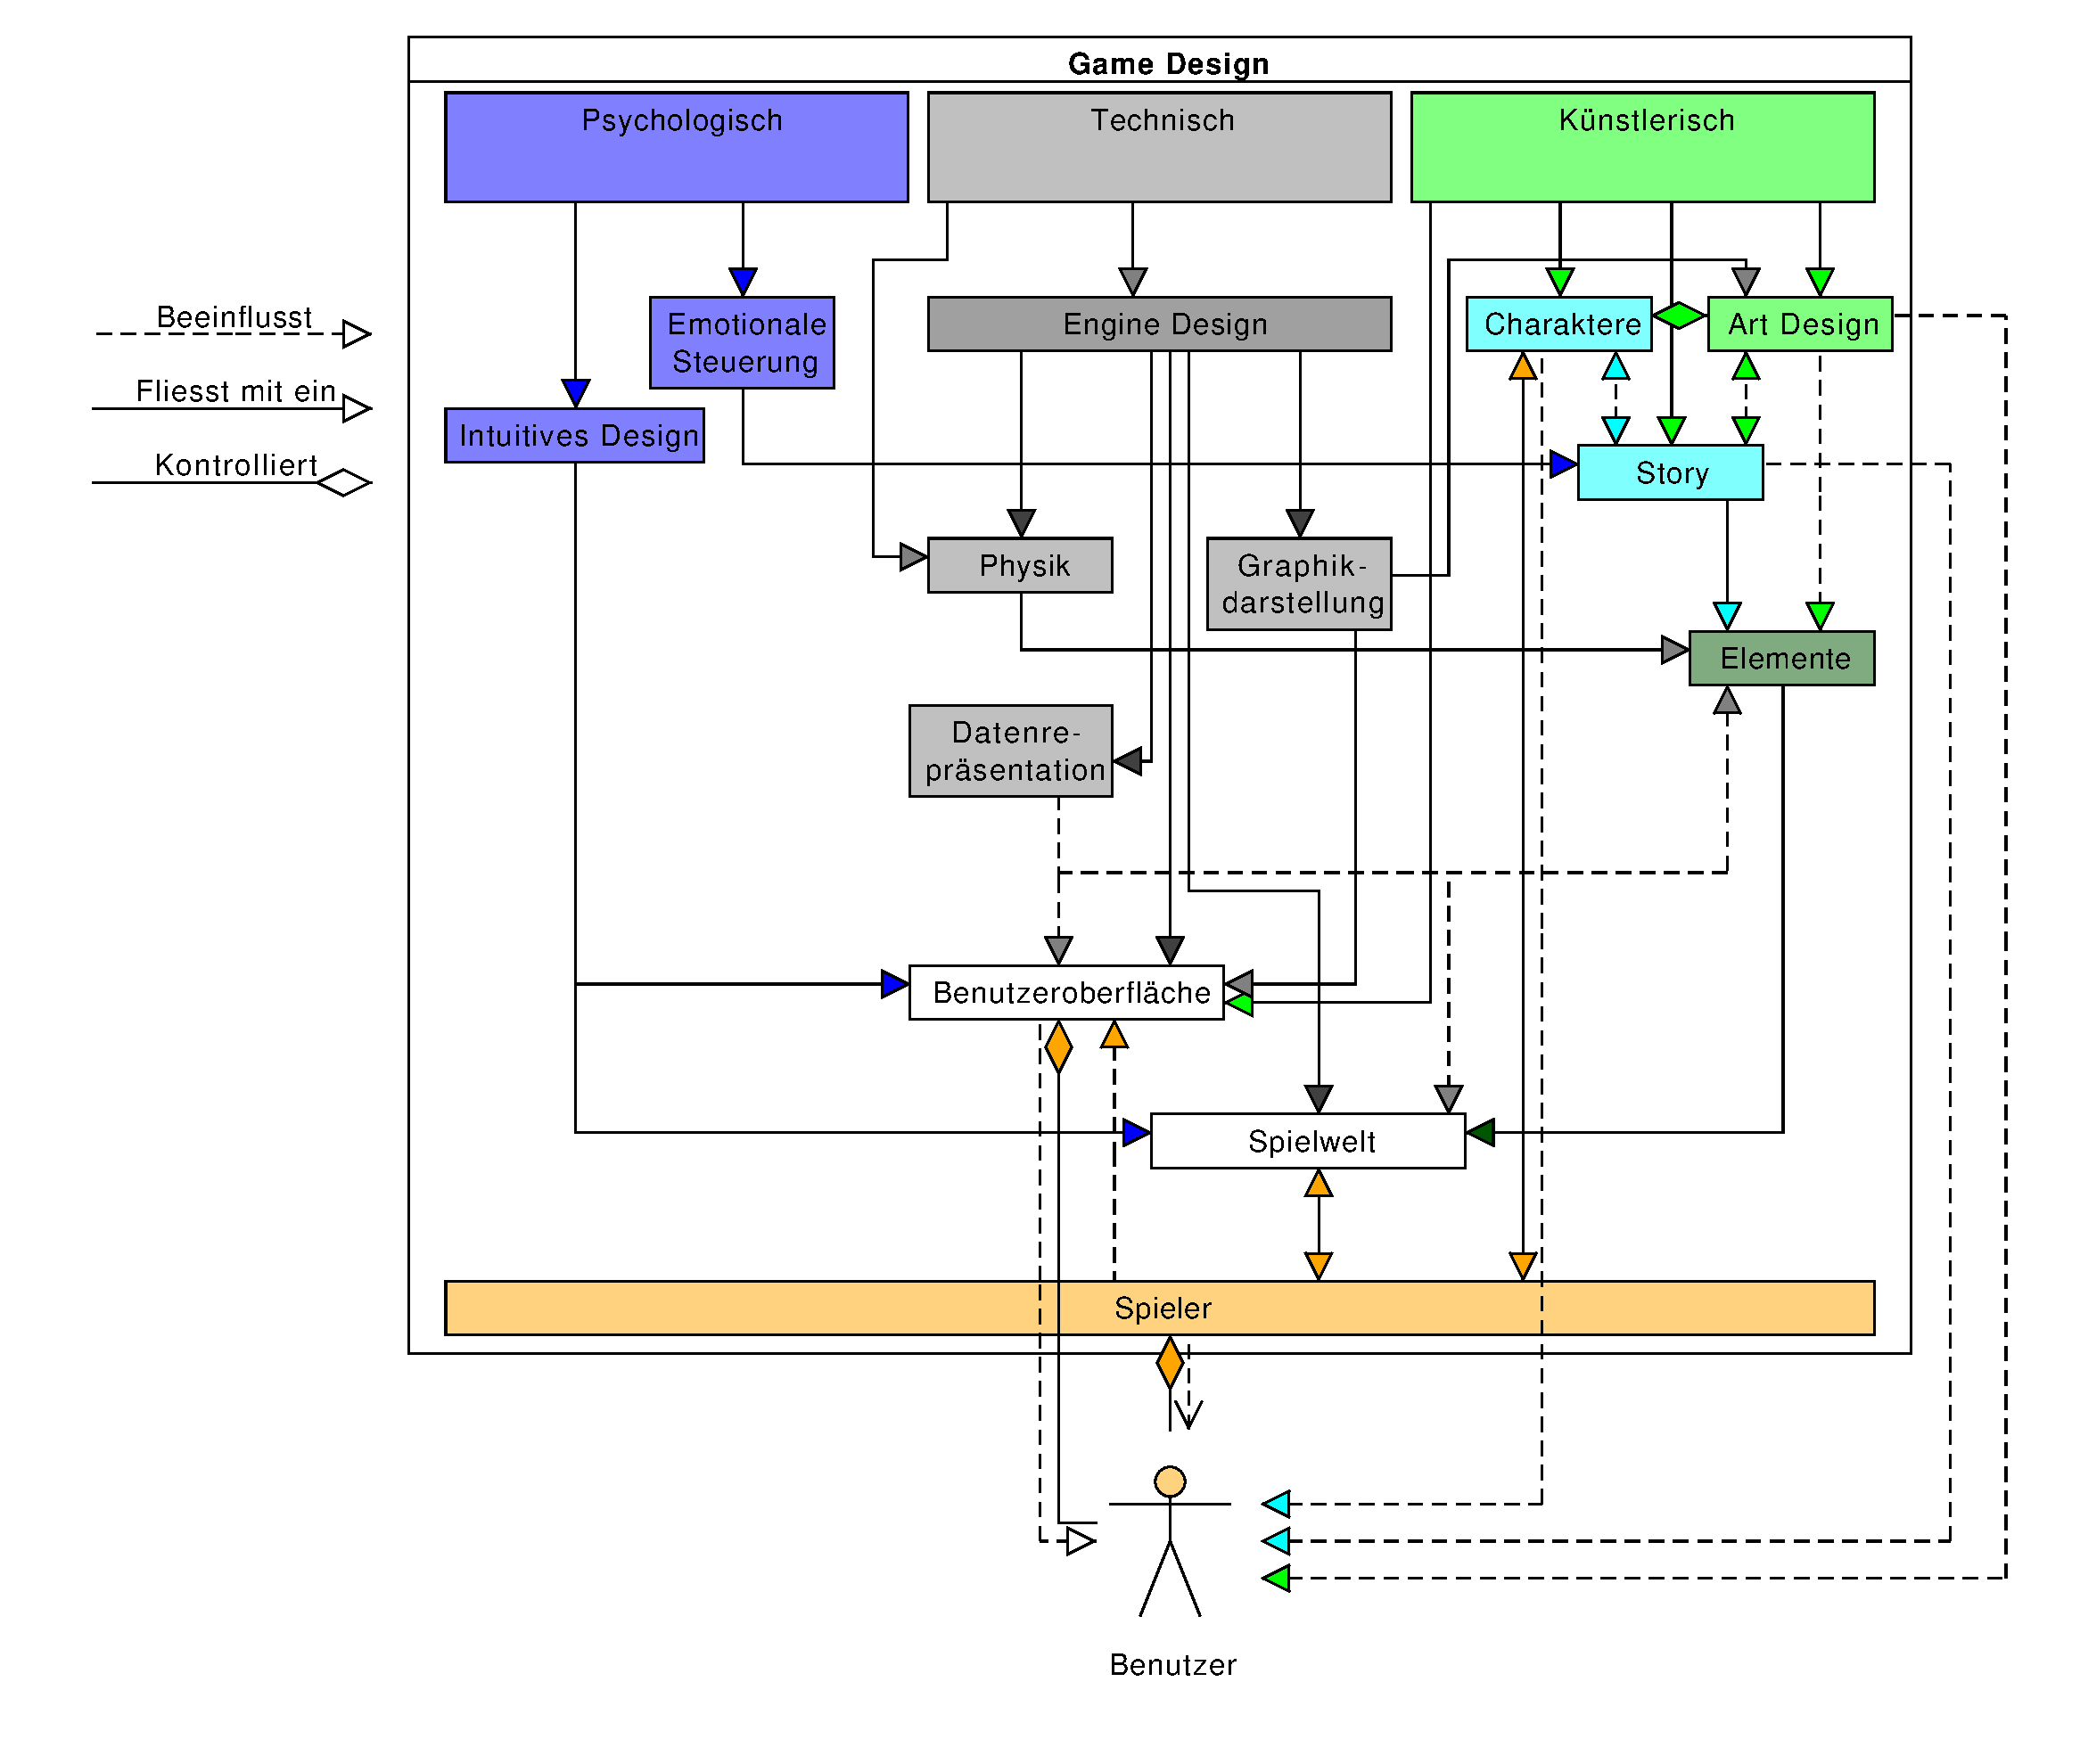
\includegraphics[keepaspectratio=true,scale=0.4]{gamedesign.pdf}
  			\caption{Darstellung einiger Bereiche des Game Designs}
		\end{figure}
		Um alle diese Bereiche zu decken ist ein enormes Wissen notwendig. Viele der Bereiche können auch nur durch ständiges Ausprobieren und Testen perfektioniert werden, was viel Zeit beansprucht.\\
		
		In meiner Arbeit habe ich mich vor allem auf das Technische konzentriert, versuchte aber dennoch auf die anderen Bereiche einzugehen und habe mich ausgiebig über sie informiert.\\
		Auch wenn im praktischem Produkt nicht auf alles eingegangen werden konnte, da es aus zeitlichen Gründen nicht reichte, werden dennoch fast alle diese Aspekte in diesem Dokument zumindest kurz behandelt.
		Dabei geht es um psychologische, anthropologische, mathematische, physikalische, künstlerische und musische Überlegungen und Konzepte, die alle beim Game Design eine Rolle spielen.
	
	\subsection{Konzepte}
		%What kind of elements, ideas and concepts did I originally have
		Als ich mit dem Projekt begann habe ich mir vor allem Dinge überlegt, die erst sehr spät im Prozess zum Einsatz kommen. So hatte ich Ideen für Spielkonzepte, eine Story und einige Grundcharaktere. 
		Das Wichtigste dabei war mir, dass das Spiel zweidimensional (2D) ist und einen Jump \& Run (J\&R) Ansatz wie z.B. Super Mario oder Sonic the Hedgehog verfolgte.
		Allerdings ist dies ja nicht eine so originelle Idee, weshalb ich mir einige Spezialitäten überlegen musste.\\
		
		Auf der Suche nach neuen Ansätzen, dachte ich zurück an Spiele, die mir selbst sehr gut gefielen. Am stärksten trat dabei Okami\footnote{\url{www.okami-game.com/}} hervor. Daraus habe ich auch das Konzept der Fähigkeiten übernommen. Damit meine ich, dass der Spieler über den Verlauf des Spiels neue Fähigkeiten erlangt, die er dann benutzen kann um neue Regionen in der Welt zu erreichen, die er vorher noch nicht erreichen konnte. Dies ist im starken Kontrast zu herkömmlichen J\&Rs, wo einem alle Fähigkeiten (bis auf sogenannte Power-ups) von Beginn an verfügbar sind. Des weiteren erlaubt dieses Konzept einen weitaus grösseren Grad an Komplexität und Wiederspielbarkeit\footnote{Das Spiel bleibt auch nach mehreren Durchläufen interessant}. So steht dem Spieler die ganze Welt von Anfang an offen, was ihm erlaubt, sie ausgiebig auszukundschaften und sich schon im voraus Gedanken zu machen, was später einmal möglich sein wird oder interessant sein könnte.\\
		
		Im Unterschied zu Okami, in welchem die Fähigkeiten nur limitierten Einfluss haben, hatte ich die Idee, dass jede Fähigkeit seine eigenen Vorteile und Nachteile bringen sollte, um den Spieler mehr zum denken anzuregen. So kam ich auf den Schluss, dass es am interessantesten wäre, dieses Konzept mittels "Formen" einzuführen. Die Verschiedenen Formen würden dem Spieler klar signalisieren, dass der Charakter nun anders zu steuern ist und für andere Aufgaben gemacht ist. Dies bringt ein RPG\footnote{Role Playing Game, ein Rollenspiel wie z.B. Final Fantasy}-ähnliches Element mit ins Spiel. Allerdings resultiert daraus auch eine anspruchsvolle Aufgabe für den Gamedesigner, da es sehr schwierig ist, Fähigkeiten und Charakter zu balancieren, sodass nicht eine Form langweilig, mühsam oder unangenehm wird, sondern alle Formen in einer Weise nützlich erscheinen und keine überwiegt. Im Kapitel 4 wird näher auf dies eingegangen.\\
		
		Wie immer in der Entwicklung von Programmen und Kunstwerken ändert sich während dem Prozess sehr vieles sehr stark und kaum etwas geht vollständig nach Plan. So hatte ich z.B. viel weniger Zeit für die Engine eingeplant, als ich dann schlussendlich benötigte. Auch stellten sich einige Ideen als unpraktisch oder nutzlos heraus und wurden wieder entfernt. Umgekehrt kamen auch viele neue Dinge hinzu, auf die ich anfangs nie gekommen wäre.\\
		

\section{Enginedesign \& Programmierung}
	\subsection{Einführung}
		%Engine is core part, handles resources and so on.
		%Does base calculations, is what makes the game run.
		%Abstraction layers between core engine and game engine
		Das Wort "engine"\footnote{Engine bedeutet Maschine, Motor oder Antrieb. Es ist die Grundlage für ein Spiel} wird sehr oft gebraucht, aber viele wissen gar nicht, was denn eine Engine überhaupt beinhaltet. Der Begriff ist auch zu einem gewissen Grad etwas schwammig, aber man kann dennoch einige Bereiche klar definieren. Die primäre Aufgabe einer Engine ist, eine Abstraktion zwischen reiner Programmierarbeit und dem eigentlichen Spielerstellungsprozess herzustellen. Dies bedeutet, dass der Game Designer nicht das ganze System in und auswendig kennen muss, sondern ein bestimmtes Set an Werkzeugen und Programmen zur Verfügung hat, die ihm das Erstellen erleichtern. Abstraktion ist generell ein wichtiges Prinzip im Objekt Orientierten Programmieren (OOP), da es viele Dinge stark vereinfacht und eine grosse Last von den Entwicklern nimmt.\\
		
		Genauer ist die Engine für die Verwaltung von jeglichem Datentransfer, für alle direkte Datenverarbeitung und die Implementation von einem Toolkit\footnote{Ein "Werkzeugkasten" mit vielen hilfreichen und oft gebräuchlichen Funktionen} verantwortlich. Dazu gehört das Speichern und Laden von Spielständen, Leveldateien, Figuren, Texturen, Graphiken, Animationen etc., sowie die Verarbeitung aller im Spiel enthaltenen Objekte, die Erkennung von Interaktionen zwischen Objekten (hauptsächlich Kollisionen), das Empfangen von Benutzereingaben, die Darstellung auf dem Bildschirm, das Ausführen von Skripten, die Ausgabe von Geräuschen und Musik, Netzwerkverwaltung, Künstliche Intelligenz (KI), Gegner und vieles mehr. Natürlich beinhaltet nicht jede Engine all diese Teile (die von mir entwickelte "Transcend Engine" hat z.B. keine Netzwerkunterstützung), aber der Grossteil davon muss vorhanden sein.\\
		
		Eine Engine kann auch in einzelne Teile unterteilt sein. So geschieht es in der Praxis auch oft, dass verschiedene Teile von verschiedenen Engines kombiniert werden. Vor allem Physik und Graphik Engines werden häufig separat entwickelt, da sie sehr grosse Komponenten sind, die viel Fachwissen und spezialisierte Arbeit verlangen.
		
	\subsection{Techniken \& Tools}
		%Explanation of OGL/AL, LWJGL, etc.
		%Thoughts about loading resources, resource management and sharing.
		Eines meiner Grundprinzipien war, alles möglichst von Grund auf selbst zu machen und so wenig wie möglich Libraries\footnote{Libraries vom Englischen bedeutet soviel wie Bibliothek und ist meist eine Sammlung von Werkzeugen und Funktionen oder eine Abstraktionsebene zum vereinfachten Zugriff auf Objekte, Geräte etc.} und Werkzeuge von Dritten zu benutzen, um so viel wie möglich über die Themen zu lernen. Allerdings muss man doch immer mit einem Fundament anfangen (solange man nicht alles in Assembler\footnote{Direkte, sehr elementare Computersprache} schreibt). 
		Dafür habe ich die standard Java SE Library, die LWJGL\footnote{Light Weight Java Game Library} und die Slick-util Library benutzt. Die Java SE Library ist ein Grundbestandteil, ohne welchen man gar nicht Java Programme schreiben könnte. LWJGL stellt eine Schnittstelle zu OpenGL\footnote{Open Graphics Library, ermöglicht 2D und 3D beschleunigte Darstellung auf dem Bildschirm} und OpenAL\footnote{Open Audio Library, ermöglicht die Ausgabe von Ton} her. Slick-util gibt nur eine einfache Klasse zum Laden von Texturen und Audio Dateien.\\
		
		Der Rest ist von Grund auf selbst programmiert und beinhaltet unter anderem Kollisionserkennung, Animation, KI, Spielstandverwaltung, Darstellungseinstellungen, GUI\footnote{Graphical User Interface, die Benutzeroberfläche}, Level Editor, Ressourcenverwaltung und mehr. Auf einige der Techniken werde ich noch genauer im Kapitel 2.5 eingehen.\\
		
		Ich habe als Programmiersprache Java gewählt, da ich schon viele Jahre Erfahrung damit habe und viele verschiedene Projekte basierend auf Java erstellt habe. Es ist auch heute noch von allen Sprachen die ich gelernt oder ausprobiert habe, mein Favorit. Weiterhin ermöglicht Java eine einfache Distribution der Software auf alle Betriebssysteme (Windows, Linux, Mac Os X, Solaris, etc.). Als Grafikbibliothek habe ich OpenGL gewählt, da die Java Bindings\footnote{Java unterstützt von sich aus OpenGL nicht, weshalb eine art Brücke (Binding) zu OpenGL benutzt werden muss.} für OpenGL (LWJGL) relativ gut und schnell funktionieren.
		
	\subsection{Ziele \& Einsatzmöglichkeiten}
		%Base 2D environments
		%2D games
		Die Transcend Engine wurde mit dem Ziel entwickelt, einen soliden Grundbaustein für beliebige 2D-Spiele zu liefern. Dabei sollte der Entwickler einen hohen Grad an Abstraktion haben, aber dennoch in Spezialfällen volle Kontrolle über das System erlangen. Folgende Punkte waren mir besonders wichtig:
		\begin{itemize*}
			\item Dynamisches Levelspeicherformat
			\item Einfach zu adaptierende Grundklassen zur Erstellung von Gegnern, Spielern und Weltelementen
			\item Speichern und Laden von Spielständen
			\item Automatisierung von Animation
			\item Einfache Ressourcenverwaltung
			\item Kollisionserkennung für primitive und komplexe Formen
			\item Eine Scriptsprache zum direkten Manipulieren vom Spielverhalten
			\item Ein Partikelsystem zur Erstellung von Effekten, wie z.B. Feuer oder Regen
			\item Eine extensive GUI und HUD\footnote{Heads Up Display, zur Darstellung von Spielinformationen wie Leben, Punkte usw.}
			\item Einfache Handhabung der Benutzereingabe durch ein Event-basiertes System
			\item Austausch von Information zwischen Spielobjekten indirekt über ein Event System
			\item Level Editor, der die Erstellung und Veränderung von Welten direkt im Spiel ermöglicht
			\item Ein System, das nicht all zu komplex und wirr zum Verwalten wird
			\item Einbindung des NexT/Package Systems, um automatische Updates zu ermöglichen
		\end{itemize*}
		Von diesen Punkten habe ich alle, bis auf das Partikel System, erfolgreich durchgeführt und in die Engine eingebunden. Sie ist von dem her für jegliches 2D Spiel einsetzbar und beschränkt sich nicht auf ein bestimmtes Spiel oder Genre. Weiterhin profitiert die Engine von Java's Eigenschaften und kann deshalb praktisch ohne jegliche Anpassung direkt auf jedem Betriebssystem ausgeführt werden.\\
		
		Ein hoher Grad an Einsatzmöglichkeiten hat auch immer seinen Preis. Dieser Preis ist ein erhöhter Zeitaufwand auf Seite des Spielentwicklers, da er mehr Funktionen selbst schreiben muss. Allerdings wird dieser zusätzliche Aufwand stetig abnehmen, je mehr die Engine wächst und je mehr Funktionen und Klassen hinzukommen.
		
	\subsection{Codedesign}
		Im Folgenden werde ich die einzelnen Konzepte und Klassen\footnote{Im OOP ist eine Klasse ein abstraktes Modell zur Bündelung von verschiedenen Funktionen und Variablen} im Detail besprechen. Das nachstehende Diagramm ist eine vereinfachte Darstellung der Interaktion der verschiedenen Hauptklassen in der Transcend-Engine.
		\begin{figure}[H]
  			\centering
			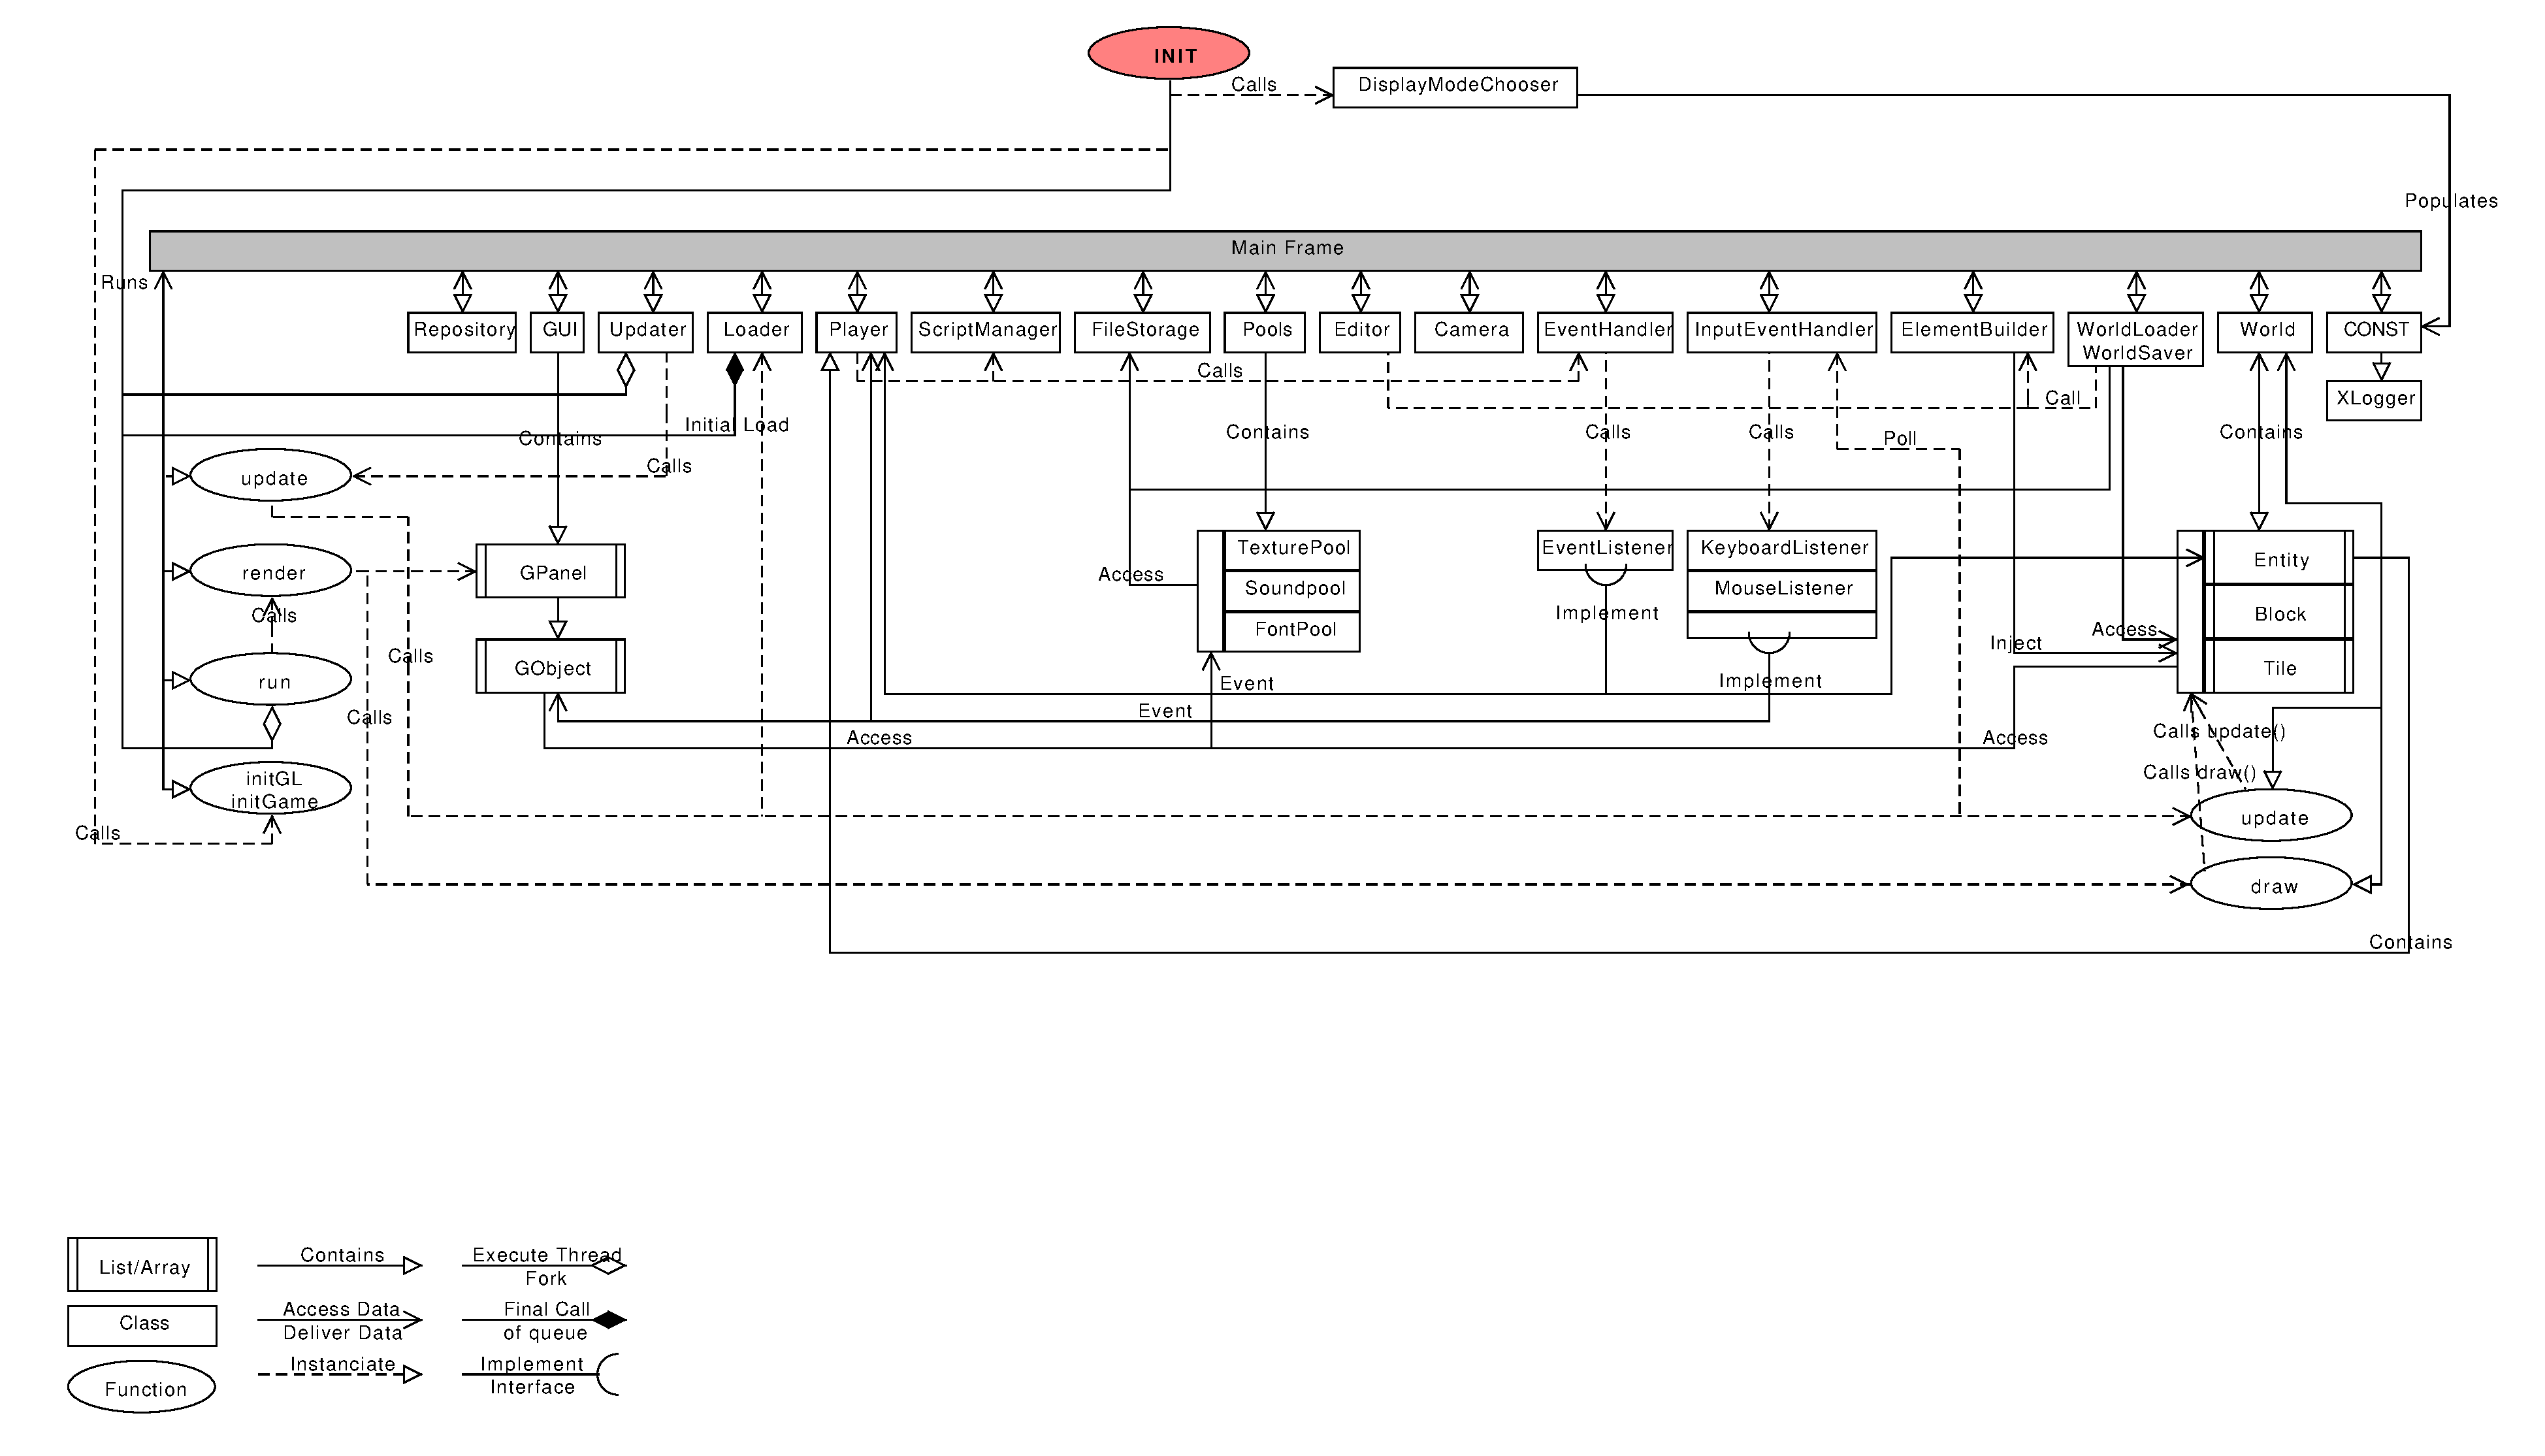
\includegraphics[keepaspectratio=true,angle=-90,scale=0.335]{transcend-engine.pdf}
  			\caption{Vereinfachte Darstellung der Transcend-Engine}
		\end{figure}
		Am wichtigsten ist dabei die MainFrame Klasse, die auch die Schnittstelle zu allen Informationen in der Engine darstellt. Ihre init Funktion startet das Programm auf, erstellt alle notwendigen Instanzen\footnote{Wichtig ist hier der Unterschied von Klassen zu Instanzen. Man kann nicht direkt auf die Variablen oder Funktionen von Klassen zugreiffen, sondern muss zuerst eine Instanz von ihnen erstellen}, setzt alle benötigten Variablen und Konstanten und übergibt schlussendlich die Kontrolle an zwei asynchrone Threads\footnote{Ein Thread ist eine kontinuierlich verarbeitete Funktion, die gleichzeitig mit anderen Threads ausgeführt werden kann. Jedes Programm benötigt mindestens einen Thread, um zu funktionieren. Mehrere Threads nennt man Multithreading oder Multitasking}, der Erste hat die Aufgabe, den Bildschirm in einem konstanten Tempo neu zu zeichnen und der Zweite die Aufgabe alle update Funktionen der Klassen aufzurufen, damit diese ihre Position und Eigenschaften verändern können. Dies erlaubt es auch, die Anzahl an FPS\footnote{Frames Per Second, Anzahl Bilder pro Sekunde} zu ändern, ohne das eigentliche Spieltempo zu beeinflussen.\\
		
		Weiterhin sehr wichtig ist die World Klasse. Ihre Instanz erhält auch die meisten Zugriffe von allen Objekten im System. Ihre Aufgabe ist die Verwaltung von allen Spielelementen, die dynamische Erstellung und Vernichtung der Elemente und die Vergabe von UIDs\footnote{Unique ID, eine einzigartige Identifikationsnummer}. Das eigentliche Laden und Speichern von Weltdateien ist eine Aufgabe der WorldLoader Klasse. Sie liest dabei eine Datei vom Computer ein und verwandelt die Textangaben in Befehle zur Erstellung der erwünschten Objekte. Diese Befehle werden dann an den ElementBuilder weitergeleitet, welcher das passende Objekt erstellt und direkt in die World Instanz einspeist. Beim Speichern der Welt wird der Zwischenschritt über den ElementBuilder aber übersprungen und die Werte werden direkt aus der World ausgelesen, in das richtige Format verwandelt und als Datei abgelegt.\\
		
		Der InputEventHandler fragt mit jedem Step\footnote{Ein Aufruf aller update Funktionen wird "Schritt" genannt} die Tastatur und Maus ab und wertet deren Eingabesignale aus. Die resultierenden Instruktionen werden dann an alle KeyboadListeners (zur Tastaturabfrage) und alle MouseListeners (zur Mausabfrage) weitergeleitet. Damit also eine Klasse diese Signale empfangen kann, muss diese einen KeyboardListener oder MouseListener implementieren und ihn beim InputEventHandler registrieren. Einen Grossteil der Aufgabe in diesem System, die eigentliche Kommunikation mit dem Betriebssystem um die Geräte abzufragen, übernimmt hier LWJGL, welches einige Klassen dafür zur Verfügung stellt. Diese Aufgabe wäre sonst sehr komplex und zeitaufwendig, da man sich auf betriebssystemspezifische Funktionen verlassen müsste und deshalb für alle Systeme eigenen Code schreiben müsste.\\
		
		Der EventHandler übernimmt alle Kommunikation von Events zwischen den Objekten in der Spielwelt. Das System funktioniert ähnlich wie das des InputEventHandlers, wobei hier der Ursprung der Events nicht der Benutzer ist, sondern andere Objekte in der Spielwelt selbst. So kann das Spieler-Objekt z.B. signalisieren, dass es gerade ein feindliches Objekt gesichtet hat, und alle Objekte die sich an dieser Information interessieren, können sich beim EventHandler registrieren. Dies ist vor allem nützlich, wenn z.B. der Spieler angreift und ein anderes Objekt berührt. Damit dies bemerkt werden kann, muss ein Kollisionstest durchgeführt werden. Kollisionstest können sehr zeitaufwendig sein. Hier kann Rechenzeit gespart werden, indem der Spieler ein Berührungs-Event aussendet, das berührte Objekt darauf hört und so nicht gleichzeitig nochmals einen Kollisionstest für sich ausführen muss. Dieses System ist ausserdem nützlich, wenn nur ein bestimmter Typ von Objekt angesprochen werden soll.\\
		
		Die verschiedenen Pool Klassen sind für die intelligente Ressourcenverwaltung zuständig. Sie stellen sicher, dass eine Ressource nur einmal geladen wird und alle Klassen auf die gleiche Ressource zugreifen. Anderenfalls würde der Speicheraufwand enorm, da alle Texturen, Töne und Schriftarten mehrere Male geladen werden müssten, auch wenn sie Duplikate sind.\\
		
		Die Player Klasse ist im Grunde genommen eine ganz normale Entity Klasse\footnote{Entities repräsentieren alle beweglichen Objekte im Spiel, darunter auch der Spieler und die Gegner}. Sie bekommt einen Spezialplatz, da sie eine so zentrale Rolle im Ganzen spielt.\\
		
		Die Loader Klasse stellt einen Ladebildschirm zur Verfügung und ist für das korrekte laden der benötigten Ressourcen zuständig. Die Instanz dieser Klasse wird auch bei Beginn des Programms aufgerufen, um den Menübildschirm zu laden (was im Grunde genommen eine leere Welt mit fixem Menü ist). Das Laden von Ressourcen kann oftmals problematisch sein, wenn es in verschiedenen Threads passiert: Wenn ein Thread versucht auf eine Ressource zuzugreifen und diese noch nicht fertig geladen ist, kommt es zu Störungen. In LWJGL und Slick-Util ist dieses Problem so gelöst, dass alle Zeichenarbeit und jegliche Ladungsvorgänge strikt in nur einem Thread passieren dürfen. Deshalb müssen also alle Ressourcen am Anfang einer neuen Welt geladen werden, damit der Spieler nicht mitten im Spiel plötzlich warten muss, bis neue Texturen geladen sind. Der Nachteil dabei ist, dass man z.T. Ressourcen laden muss, die später gar nie benötigt werden, oder nur für eine kurze Zeit. In komplexeren und fortgeschritteneren Engines wird übrigens dieses Singlethreading System nicht angewendet und Ressourcen können während dem Spiel geladen werden.\\
		
		Alle anderen Klassen, die im Diagramm abgebildet sind, erfüllen nur kleinere Funktionen, auf die ich hier nicht eingehen möchte. Zudem gibt es in meiner Engine noch viele weitere Klassen, die gar nicht erst auf dem Bild vorkommen. Für eine komplette Liste der Klassen muss ein Blick auf den Sourcecode\footnote{Die Dateien, die den eigentlichen Programmiercode enthalten} geworfen werden.
		
	\subsection{Probleme im Detail}
		In diesem Bereich werde ich auf einige wenige der Probleme auf die ich während dem Programmieren gestossen bin, etwas näher diskutieren und behandeln.
		
		\subsubsection{Kollisionserkennung}
			Kollisionserkennung ist eine der wichtigsten Aufgaben einer Gameengine und repräsentiert auch oft ein Flaschenhals\footnote{Ein Teil wird als Flaschenhals bezeichnet, wenn er langsam ist und diese Performanceschwäche das ganze System beeinflusst}. Es gibt eine Unmenge and verschiedenen Algorithmen, Techniken und Konzepte mit variierender Komplexität, Leistung und Genauigkeit.\\
			
			Zur Zeit sind in der Transcend-Engine eine Simple Box-Kollisionserkennung und eine Linien-Strahlen-Kollisionserkennung implementiert. Die erste ist die schnellst mögliche Kollisionsprüfung, da sie sehr wenige und sehr einfache Berechnungen verlangt. Die zweite ist zur genauen Erkennung eines Kollisionspunktes von zwei Geraden oder einem Strahl und einer Geraden. Diese Überprüfung ist immer noch relativ einfach zu lösen, da sie nur simple Vektorgeometrie benötigt.
			\begin{figure}[H]
  				\centering
				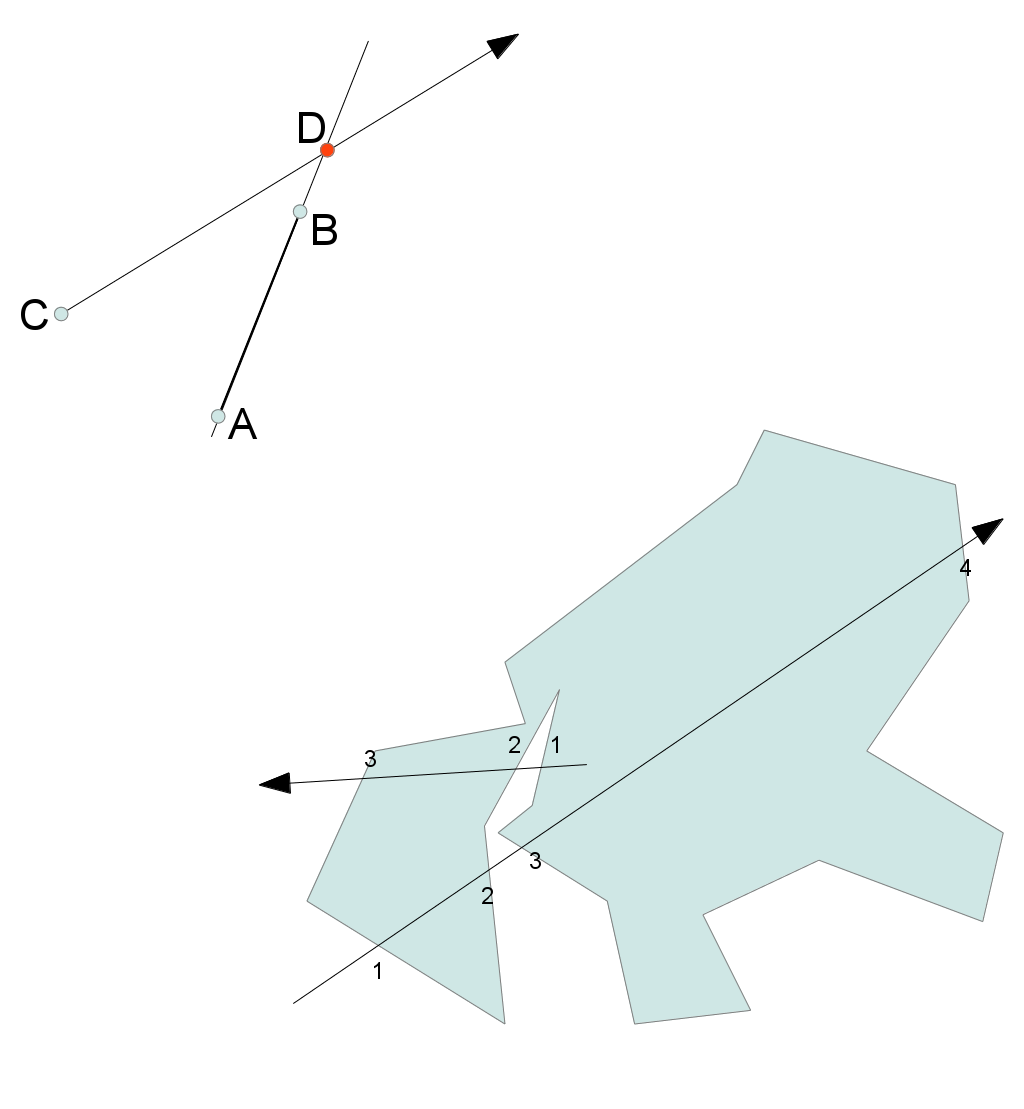
\includegraphics[keepaspectratio=true,scale=0.3]{collision.png}
  				\caption{Linienschnittberechnung und Gebietsprüfung}
			\end{figure}
			Da wir aber nicht Geraden überprüfen wollen, sondern Strecken (z.B. Polygonseiten), müssen wir das Verfahren etwas ändern. So werden die Linie und der Strahl zu Geraden erweitert und der Abstand von einem Endpunkt der Strecke zum erkannten Schnittpunkt (falls dieser existiert) berechnet. 
			$$u=\frac{\vec{r}_y*(A_x-\vec{r}_x)-\vec{r}_x*(A_y-\vec{r}_y)}{\vec{r}_y*(A_x-B_x)-\vec{r}_x*(A_y-B_y)}$$
			$$\vec{r}_x > \vec{r}_y : t=\frac{A_x-\vec{r}_x+(B_x-A_x)*u}{\vec{r}_x}$$
			$$\vec{r}_x < \vec{r}_y : t=\frac{A_y-\vec{r}_y+(B_y-A_y)*u}{\vec{r}_y}$$
			Falls dieser Abstand grösser ist, als die Länge der Strecke, so liegt der Schnittpunkt ausserhalb und ist deshalb nicht Teil der Lösungsmenge. Die berechnete Zahl der Funktion gibt den Abstand zum Ursprung des Strahls an. Ist diese Zahl negativ, so liegt der Punkt auf der entgegengesetzten Seite des Strahls und ist deshalb keine Lösung. Ist der Punkt allerdings in der Lösungsmenge enthalten, so lässt sich mit der berechneten Zahl und dem Ursprung sehr leicht der eigentliche Schnittpunkt berechnen.\\
			$$D=\begin{pmatrix}C_x+\vec{r}_y*t\\C_y+\vec{r}_y*t\end{pmatrix}$$
			Zweidimensionale Objekte können durch Polygone repräsentiert werden. Um nun zu überprüfen, ob ein Strahl innerhalb oder ausserhalb eines Polygons liegt, verwendet man eine spezielle mathematische Eigenschaft: Ein Strahl dessen Ursprung innerhalb einer komplexen Figur liegt (die Figur darf sogar löcher enthalten) hat immer eine ungerade Zahl an Schnittpunkten, während ein ausserhalb liegender Punkt immer eine gerade Anzahl hat. Dies ist im zweiten Teil der Abb. 3 illustriert.
			
		\subsubsection{KI}
			Künstliche Intelligenz ist in Spielen ein sehr wichtiger Aspekt und hat einen enormen Einfluss auf das Spielverhalten hat. Die "künstlichen" Gegner dürfen nicht zu intelligent und nicht zu simpel sein. Weiter ist das Zusammenspiel der verschiedenen Gegnertypen sehr wichtig. Eine gute KI zu bilden ist deshalb sehr schwierig und erfordert viel Aufwand.\\
			
			In den älteren, bekannten J\&R spielen wie Super Mario und Sonic sind die Gegner sehr einfach und direkt gestaltet. Meistens laufen sie einfach hin und her und reagieren kaum auf Spieler. Sie haben keine lernende oder zufallsgesteuerte Intelligenz. In solchen Fällen ergibt sich der Schwierigkeitsgrad des Spiels aus der Konstellation der Gegner und dem Leveldesign.\\
			
			Warum sind nur Gegner im Spiel vorhanden, die einfache, festgesetzte Regeln befolgen? Einerseits gibt dies Vorteile von der Entwicklung und vom Gamedesign her, andererseits ist es in einem Platformer praktisch unmöglich, eine gute Pfadsuche für die künstlichen Gegner zu erstellen.
			\begin{figure}[H]
  				\centering
				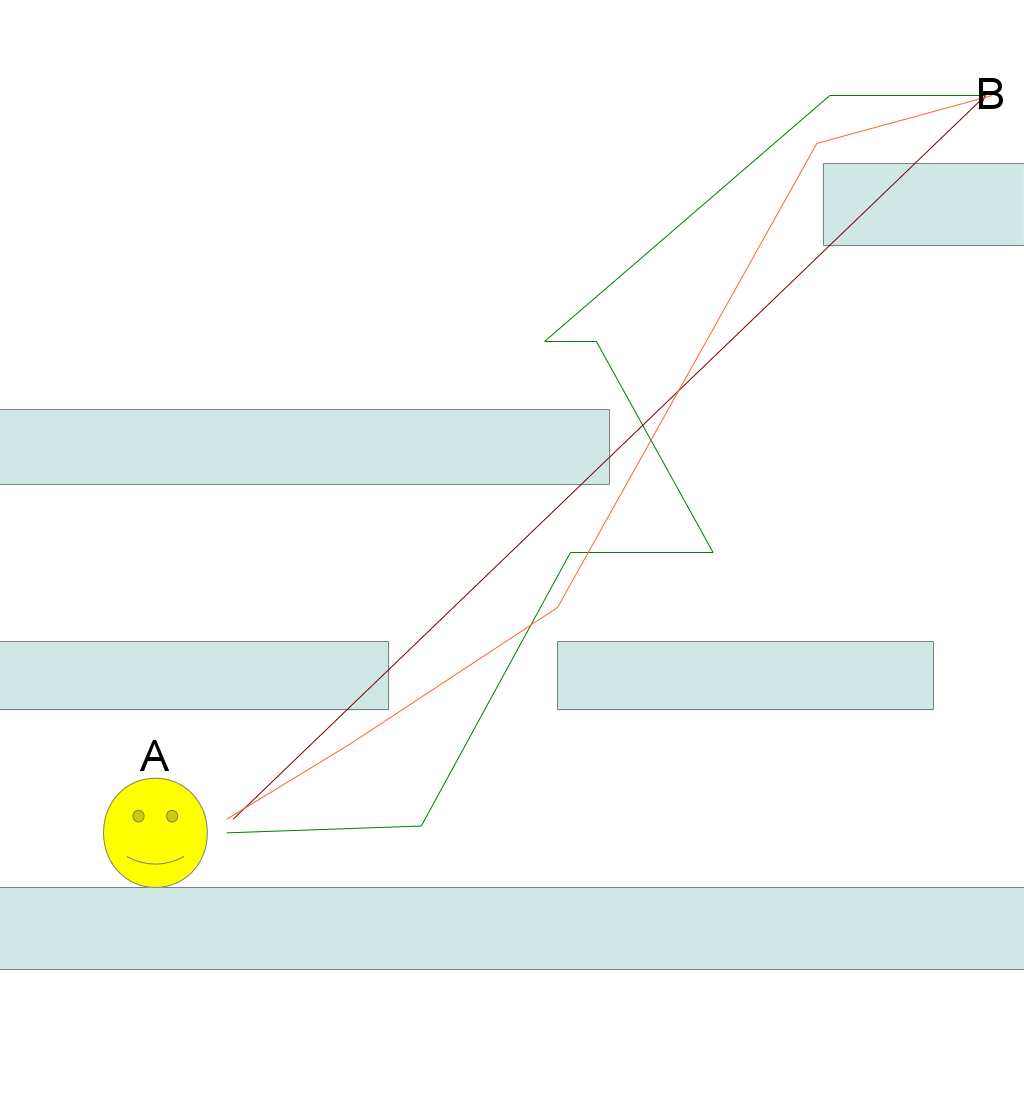
\includegraphics[keepaspectratio=true,scale=0.3]{ai.png}
  				\caption{Darstellung des Problems der Pfadfindung bei Plattform Spielen}
			\end{figure}
			Es gibt einige Algorithmen zur Pfadfindung, diese werden meist zur Bewältigung von Labyrinthen oder Ähnlichem gebraucht. Der direkte Weg wird in der Darstellung durch die rote Linie repräsentiert. Dieser kann aber nicht begangen werden, da andere Plattformen im Weg stehen. Die orange Linie zeigt den Weg, den ein normaler Pfadfindungsalgorithmus vorschlagen würde. Allerdings funktioniert dies nicht immer, wenn z.B. die Figur nicht hoch genug springen kann, um B direkt zu erreichen. Ausserdem würde dieser Pfad eher dem eines fliegenden Gegners gleichen. Deshalb ist eine solche Methode unbrauchbar.\\
			
			Stattdessen muss ein Ansatz mit Hilfe von KI angewendet werden. Dies funktioniert vor allem durch die Erkennung von Aktionsmöglichkeiten (gehe links, gehe rechts, springe links, etc.) und der Erfolgswahrscheinlichkeitsberechnung. So werden Aktionen, die einen Gegner näher zum Ziel bringen, eine höhere Wahrscheinlichkeit haben, als solche, die ihn weiter weg bringen. Allerdings ist es eben auch nötig z.T. zuerst einen Schritt in die falsche Richtung zu machen, vor allem wenn der Charakter an Höhe gewinnen sollte. Ein solcher komplizierter Ansatz funktioniert für einfache Szenarien gut, ist aber in komplexen Situationen schnell überfordert und benötigt einen hohen Optimierungsaufwand.
			
		\subsubsection{NexT/Script}
			Praktisch alle modernen Spiele benutzen eine interne Scriptsprache, um einige der Berechnungen durchzuführen. Dies bringt den Vorteil, dass man während dem das Spiel läuft, direkt Eigenschaften und Verhalten ändern kann. Auf konventionelle Weise, ohne Scriptsprache, muss man dies alles direkt im Programm deklarieren. Jedes mal wenn etwas geändert wird, muss das ganze Spiel neu kompiliert, gestartet und überprüft werden. Die Möglichkeit alle diese Schritte zu überspringen, bringt dem Entwickler einen enorm grossen Komfort und Entwicklungsgeschwindigkeitsvorteil. Natürlich hat dies auch einige Nachteile. So muss zum einen die Scriptsprache schnell genug sein, damit sie nicht zu einem Flaschenhals für das Programm wird und natürlich ist die Scriptsprache bei weitem nicht so gut integriert und umfangreich, wie die Sprache in welcher sie ausgeführt wird.\\
			
			Die Implementation der Scriptsprache in Transcend geschieht durch die Anwendung der NexT/Script\footnote{NexT/Script ist ein Unterteil der NexT Bibliothek} Bibliothek (welche ebenfalls von mir erstellt wurde). Ein Beispiel für ein Script in NSC sieht folgendermassen aus:
			\begin{lstlisting}[label=NSCEX1,caption=NexT/Script Beispiel]
				#NexT/script 
				//Befehle werden Zeile fuer Zeile angegeben, kein Delimiter
				//Kommentare koennen // fuer inline oder /* */ fuer multiline sein
				//Definiere globale script Variablen:
				a=10 //integers
				b=0.5 //doubles
				c="test" //strings
				d=true //booleans
				e={0,2,5.4,true,"whatever"} //mixed arrays
				f={{0,3,5},{{11,3,5},{"a","b"}}} //multi-dimensional arrays

				defun myFunction{ 
					temp = (+ 5 a (getRandom 0 100 ) (sin b ) ) //Mathematische Ausdruecke basierend auf LISP Syntax
					return temp //Gib eine Variable als Ergebnis zurueck
				} 

				defun getRandom{ //Argumentvariablen werden nicht spezifiziert
					rand = (+ (floor (* (rand) $1 ) ) $0 ) 
					return rand
				}
			\end{lstlisting}
			Intern werden Variablen in einem speziellen Objekttyp repräsentiert, der viele verschiedene Formen annehmen kann und sogar multidimensionale Listen repräsentieren kann. Funktionen werden mit "defun" eingeleitet und sind mit geschweiften Klammern begrenzt. Die Argumente einer Funktion können noch nicht festgelegt werden (dies ist aber geplant). Übergebene Argumente können nur mittels \$n abgerufen werden, wobei n die Stelle des Arguments angibt. Variablen die innerhalb einer Funktion definiert werden sind nicht ausserhalb der Funktion gültig.\\
			
			Das Herzstück der NSC Sprache ist der Math-Parser. Dieser verwandelt LISP-Syntax\footnote{LISt Processing ist eine spezielle Programmiersprache} ähnliche Zeichenketten in eigentliche Befehle. Dabei ist die Syntax für einen Funktionsaufruf sehr einfach definiert: (funktionsname argument1 argument2 argument3 ... argumentn). Sogar einfache Operationen, wie die Addition, werden in LISP als Funktionen betrachtet z.B steht (+ 5 2 ) für 5+2. Die übergebenen Argumente können ihrerseits wieder Funktionsaufrufe sein. Ein weiteres Beispiel:
			\begin{lstlisting}[label=NSCEX2,caption=NSC-Math Beispiel]
				#NexT/script 
				result = (+ 5 2 Pi (* 2 3) (sin 90) (def temparray {2,5,7,3}) (- (/ 2 (< temparray 0)) 1))
				print result //Gibt 17.0355893 zurueck
			\end{lstlisting}
			Der angegebene Term kann in unserer Schreibweise folgendermassen ausgedrückt werden:
			$$5+2+\pi+2*3+sin(90)+((2/temparray[0])-1)$$
			Der def Befehl wurde hier ausgelassen, da es in der Mathematik keinen Ausdruck zum definieren von Variablen innerhalb eines Terms gibt. Es ist deshalb einfach gegeben, dass temparray eine Menge mit den Elementen 2,5,7 und 3 ist. Vereinfacht gibt der Term folgendes:
			$$13+\pi+sin(90)+0$$
			Die NSCS ist noch nicht fertig entwickelt und muss noch einen langen Weg gehen, bis sie umfangreich, stabil und schnell genug ist, damit sie extensiv gebraucht werden kann.\\
			

\section{Grafikdesign}
	\subsection{Einführung}
		%Which parts does graphics design cover
		Grafikdesign befasst sich mit allen Dingen, die mit Darstellung zu tun haben. Dazu gehören Animation, Hintergrundgestaltung, Weltgestaltung, Charakterdesign, GUI Gestaltung, Spezialeffekte und Konzeptzeichnungen. Es ist von dem her das am meisten Artistisch konzentrierte Gebiet, auch wenn es sich mit einigen technischen Aspekten auseinandersetzen muss.
		
	\subsection{Ideen \& Konzepte}
		%Which thoughts have I given the character design
		%How is it incorporated in the story
		Wichtig ist, dass die Charaktere zur Story passen, miteinander verbindbar sind und den Spieler ansprechen. Sie sollten ausserdem mit der Welt zusammenpassen und mit den Hintergründen harmonieren. Allerdings muss der Spieler die Figuren trotzdem vom Rest abheben können, weshalb auch ein gewisser Anteil an Kontrast vorhanden sein muss.\\
		
		Der Spieler sollte sich klar mit der Spielfigur identifizieren können und sich von den Gegnern abheben. Kann man sich nicht in die Spielfigur einfühlen, so wirkt das ganze falsch und künstlich. Gibt es nur geringen Unterschied zwischen dem Helden und den Gegnern, so wird es schwierig die zwei zu unterscheiden und die Aufgabe oder der Wunsch des Spielers, die Gegner zu besiegen, ist nicht mehr vorhanden.\\
		
		Es gibt unendlich viele verschiedene Möglichkeiten einen Charakter zu erstellen und in eine Geschichte einzubinden. Wichtig ist nur, dass die Person hinter dem Bildschirm eine Beziehung zur Figur aufbauen kann und sich ganz in die Welt des Spiels verlieren kann. Gute Spiele, wie auch Bücher können einem für Stunden in eine völlig andere Welt befördern. Das visuelle Aussehen der Welt und seiner Einwohner hat dabei eine enorm wichtige rolle und es gibt Leute, die ein Spiel vermeiden, nur schon weil ihnen der Zeichenstil nicht ganz passt.\\
		\begin{wrapfigure}{r}{8cm}
  			\centering
			
\includegraphics[keepaspectratio=true,scale=0.4]{humanform.png}
  			\caption{Die menschliche Form der Spielfigur in Transcend}
		\end{wrapfigure}
		Für mich war vor allem wichtig, dass der Spieler schnell mit den Eigenschaften und Zielen des Charakters vertraut ist und schnell und sich schnell und einfach von den Gegnern unterscheiden kann. Eine solche Einstellung passt nicht zu jeder Geschichte und es wäre auch schwierig den Charakteren so tiefe zu verleihen, da sie schon praktisch von Beginn an vom Spieler mit Ideen gefüllt werden. Es ist natürlich nicht unmöglich, würde aber eine lange Zeit und viel können vom Schreiber abverlangen. Mehr dazu im Kapitel 4.\\
		
		Um eine schnelle Assoziation zu erreichen, müssen die Motive von der Gestaltung her schnell ersichtlich sein. Der Hauptcharakter in Transcend soll eine Gottheit repräsentieren, welche auf die Erde hinabsteigt, um sie vom Bösen, welches das ganze Land überfallen hat, zu befreien. Der Die Göttlichkeit wird dabei durch das reine Weiss und die sanften Bewegungen angedeutet. Weiterhin ist das Einführungslevel aus Wolken gestaltet und der Spieler kann zusehen, wie sein Charakter auf die Welt hinabsteigt. Die Fähigkeit, seine Form beliebig zu ändern zeugt von grosser Macht und lässt auch leicht auf etwas Übernatürliches schliessen.\\
		\begin{wrapfigure}{l}{8cm}
  			\centering
			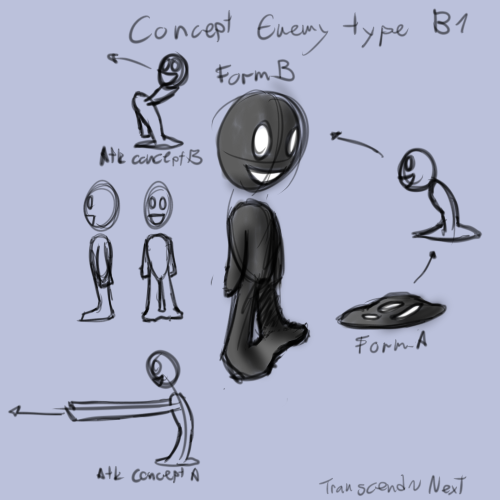
\includegraphics[keepaspectratio=true,scale=0.4]{enemy1concept.png}
  			\caption{Konzeptzeichnung eines Gegnertypen}
		\end{wrapfigure}
		Die Gegner sind stark stereotypisch. Sie sind schwarz, unrein und oft böse aussehend. Die Tinte, welches das Land überfällt wird klar als Schmutz dargestellt und die Gegner, die daraus wachsen werden von dem her relativ einfach mit dieser Verunreinigung in Verbindung gebracht.\\
		
		Die Gestalt der verschiedenen Regionen soll direkt mit den einzelnen Formen des Spielers in Verbindung gebracht werden. So gibt es eine Welt des Fliegens für die Adler Form, eine Wasserwelt für den Delphin, eine Höhlenwelt für die Maus, eine metallische Welt für den Menschen, eine erdige Welt für die Pony Form und schlussendlich eine Eiswelt für das Heimatgebiet des Bösewichten. Alle diese Welten haben ihren eigenen Stil und ihr eigenes, typisches aussehen. In jeder Welt gibt es aber auch immer wieder Elemente anderer Welten, die eingemischt wurden, um ein nicht-lineares Spielerlebnis, viel Freiheit und Entdeckungsmöglichkeiten zu bieten. Die typische Gestaltung der Welten spielt dabei eine wichtige Rolle, da der Spieler sonst nur schwer erraten kann, wo er gerade ist, wo er noch hin muss oder welchen Weg er begehen kann.
		
	\subsection{Einschränkungen}
		%Limitations by the engine
		%Time like limitations and speedups
		Im Falle der Transcend-Engine gibt es einige Limitierungen, die man beachten muss. Z.B. ist das Format der Animationen und Texturen strikt festgelegt. Die Dimensionen einer Texturdatei müssen immer eine Zweierpotenz sein. Diese Limitierung kommt von OpenGL her und hat mit der Speicherreservierung zu tun. Die Animation muss in einem Spritesheet\footnote{Tabellenartige anordnung jedes einzelnen Bildes} angelegt sein und die einzelnen Bilder dürfen nie in der Grösse variieren.\\
		
		Spezifisch für dieses Projekt musste ich die Darstellungsart vereinfachen. So sind alle Gegner rein schwarz-weiss und der Spieler rein weiss mit schwarzen Aussenlinien. Natürlich musste ich auch die Bildanzahl drastisch einschränken. Eine höhere Anzahl an Bildern pro Animation gibt eine weichere und flüssigere Wiedergabe, benötigt aber sehr viel mehr Zeit zum zeichnen, da jedes Bild einzeln erstellt werden muss. Die Formen des Hauptcharakters sind ebenfalls stark vereinfacht (deshalb dieses Gewand bei der menschlichen Form) dargestellt, um Zeit beim Animieren einzusparen.\\
		

\section{Gamedesign}
	\subsection{Einführung}
		%What is game design, how does it flow together?
		%What skills do you need for this?
		Gamedesign ist nicht nur das Erstellen von Videospielen oder Computerspielen, sondern auch das analoge Erstellen von Brettspielen, Kartenspielen usw. Es setzt sich mit dem Erstellen von Spielen jeglicher Art auseinander. Dabei wird ein breites Wissen, das in viele Bereiche wie Psychologie, Anthropologie, Ästhetik und Architektur eingeht benötigt. Allerdings kann jeder ein Gamedesigner sein, denn alle haben schon zumindest ein Grundverständnis von diesen Gebieten. Es erfordert Übung, Motivation, Engagement und Lernwille um diese Gebiete zu meistern und das nützlichste für das Gamedesign daraus abzuleiten.\\
		
		Spiele sind etwas grundlegendes für uns Menschen. Wir lernen von unseren Kindesjahren bis ins Erwachsenenalter durch Spiele oder erfreuen uns an der Herausforderung, die ein Spiel bringt. Was genau ein Spiel ist, ist nur sehr schwer zu beschreiben und es gibt keine eindeutige Definition dafür. Sicher steht jedoch, dass ein Spiel eine Herausforderung darstellt und uns zum lernen Anregt (wir lernen die Regeln und Strategien des Spiels). Praktisch jede Aufgabe kann auch sehr leicht in ein Spiel umgewandelt werden. So kann eine mühsame Aufgabe in ein aufregendes Spiel verwandelt werden und gegebenenfalls sogar Spass bieten. Dies funktioniert vor allem deshalb, weil der Mensch nach einigen Grundprinzipien strebt, die das Spiel ansprechen kann.
		\begin{itemize*}
			\item Selbstverwirklichung. Der Mensch möchte sich selber entwickeln und seine Interessen befolgen, seine Ideen verbreiten.
			\item Meisterung. Wir alle möchten Aufgaben bewältigen und Probleme lösen. Wir streben danach, ein Gebiet zu Meistern oder ein Problem zu überkommen.
			\item Verbindung, Kommunikation. Verhältnisse und Verbindungen mit anderen Menschen oder Charakteren aufzubauen ist etwas Selbstversändliches, eine so tief liegende Eigenschaft, dass wir meist gar nicht merken, wenn wir uns mit Etwas oder Jemandem verbinden.
			\item Lernen. Neues aufzunehmen und zu verarbeiten ist ein weiterer, sehr essentielles Prinzip. Ohne lernen zu wollen, ohne von Neuem erfahren zu wollen könnten wir nicht leben.
		\end{itemize*}
		Es gibt noch weitere solcher Grundprinzipien und -Triebe, die den Menschen ansteuern und die ein Spiel für uns interessant machen können. Natürlich gilt es auch zu beachten, auf welche Demographie das Spiel abgesehen ist. So gibt es je nach Geschlecht und Alter verschiedene Aspekte, auf die man beim Erstellen des Spiels achten sollte.\\
		
		Gamedesign fokussiert darauf, eine möglichst gute Erfahrung zu bringen. Ein Spiel spielen bringt uns eine Erfahrung. Diese Erfahrungen sind immer subjektiv und können von Person zu Person sehr stark variieren. Dennoch gibt es einige Hilfestellungen und Leitfäden, die einem den Weg zum Erstellen einer guten Erfahrung zumindest etwas aufklären können. Gamedesign ist eine Kunst für sich, die aber sehr aufregend und interessant sein kann, vor allem wenn man selbst ein Spielenthusiast ist. 
		
	\subsection{Charakterdesign}
		%What is important for characters?
		%How do they relate tothe artwork and story?
		%What was my implementation of this, what though path did I take?
		Wie schon im Kapitel 3.2 teilweise besprochen wurde, muss der Charakter dem Spieler gefallen und er muss mit ihm eine Verbindung aufbauen können. Weiterhin müssen die Charaktere in die Story und in die Welt des Spieles hineinpassen. Dabei ist dies aber nie ein nur einseitig wirkender Einfluss, sondern die Story und die Welt richten sich ebenfalls nach den Charakteren. Dies erzeugt ein Zusammenspiel und ein konstanter Austausch zwischen der Welt und den Charakteren. Es darf also nicht geschehen, dass eines der beiden unabhängig voneinander entwickelt wird, sonst würden sie nicht zueinander passen.\\
		
		Jeder Charakter in einem Spiel nimmt eine bestimmte Rolle in der Geschichte ein. Kein Charakter sollte überflüssig oder unnötig erscheinen, da sie den Spieler nur belasten und die Entwicklung verlangsamen. Alle Charakter sollten miteinander in irgendeiner Weise verbunden sein und sich gegenseitig beeinflussen. Dadurch lassen sich die Personalitäten der Charaktere während dem Lauf der Geschichte verändern. Dies lässt sie echt und glaubwürdig erscheinen, da sie wie echte Menschen sich ständig ändern und einstellen.\\
		
		Allerdings kann bei weitem nicht jeder Charakter so flüssig und real sein, da es sonst schnell viel zu kompliziert werden würde. Hier kommen Stereotypen ins Spiel. Stereotypen sind ein enorm wichtiges Werkzeug, um eine Geschichte und Charaktere zu entwickeln, da dem Betrachter sehr schnell klar ist, was dies für eine Person oder für ein Typ ist. Dies bedeutet, dass der Charakter nicht aufwendig vorgestellt werden muss, sondern sofort zum Einsatz kommen kann. Schlecht wird es nur, wenn ein Stereotyp zu oft oder zu lange vor kommt. Dann erscheint es aufgezwungen und falsch.\\
		
		Wie schon besprochen im Kapitel 3.2, hat das Aussehen der Figur ebenfalls einen Einfluss auf den Betrachter. Deshalb ist es nicht ausser Acht zu lassen, dass das Aussehen und die Charakterzüge übereinstimmen sollten. Allerdings kann durch eine solche Unstimmigkeit (solange sie nicht zu gross ist) auch eine Spannung aufgebaut werden und so Interesse im Spieler geweckt werden. Dies ist allerdings eine delikate Sache und ist es ist schwierig es richtig hinzubekommen.\\
		
		Nicht zu vergessen ist der Aspekt der Fähigkeiten. Ein Charakter muss ausbalanciert sein. Wenn er zu schwach ist, kommt er als nutzlose Last vor und wenn er zu stark ist als ein Spielverderber. Die Fähigkeiten einer Figur sollten auch während dem Verlaufe der Geschichte geändert werden, da sie sonst nicht mehr zu den restlichen Charaktereigenschaften passen.\\
		
		Es kann auch leicht passieren, dass der Drang nach Veränderung eines Charakters zu gross ist und dann alles in einer zu kurzen Zeit geändert wird. Dies nennt man einen Charakterbruch. Die Aktionen scheinen zu irreal und unmöglich und der Charakter zerfällt ganz. Veränderungen sollten also langsam oder nur sehr leicht stattfinden.\\
		
		Die Personalität der Spielfigur in Transcend ist im Moment noch blank. Ich konnte mir noch nicht genug Gedanken dazu machen, da mir die technischen Mittel (Dialog- und Inventar System, Städte) noch fehlen und die Geschichte des Spiels noch nicht weit genug ausgereift ist.
		
	\subsection{Story}
		%Is a story relevant or necessary?
		%How does a story intervine with everything else?
		%The story I planned for this
		Eine Geschichte oder Story ist nicht nötig, um ein Spiel zu erstellen. Einfache Puzzles und Denkaufgaben können als Spiele angesehen werden, obwohl sie keine Anzeichen einer Geschichte bringen. Allerdings kann eine Geschichte ein Spiel sehr viel interessanter machen, da es eine ganz neue Ebene an Komplexität und Möglichkeiten offeriert. Speziell Kinder erfinden immer wieder Geschichten für ihre Figuren, Spielzeuge, Plüschtiere und so weiter. Geschichten verbinden uns sehr stark mit dem Medium und sind eine ganz eigene Welt, die man ewig untersuchen könnte.\\
		
		In Spielen ist die Geschichte aber noch ein Stück schwieriger zu kreieren. In Büchern folgt der Lesefluss ganz linear. Der Autor kann genau bestimmen, was wann passiert, wieso und warum. Diese Vereinfachung steht im Spiel nicht offen, da der Spieler die Geschichte bis zu einem bestimmten Grad selbst schreibt und beeinflusst. So muss das ganze viel dynamischer und breiter gestaltet sein. Ein Spiel, dessen Geschichte zu linear ist, wird schnell als langweilig und einschneidend angesehen, da es dem Spieler nicht genug Freiheit gibt. Ein gutes Mittel zwischen geleiteter Geschichte und freiem Bestimmen zu finden ist sehr schwierig und erfordert viel Ausprobieren und Übung. Die Aufgabe ist auch von Spiel zu Spiel wieder vollkommen anders, da nicht alle Spiele den selben Regeln und Mechaniken folgen und jedes Spiel verschiedene Charaktere hat.\\
		
		 Wie schon vorhin erwähnt wurde, ist die Gestaltung einer Geschichte ist im nahen Zusammenhang mit der Erstellung der Charakteren. Dies leitet vor allem daher, dass die Charaktere die Geschichte vorantreiben und den Haupteinfluss spielen. Allerdings ist dabei die Umgebung, in der die Figuren leben und agieren nicht zu vergessen. Durch z.B. einen Vulkanausbruch oder ein sonstiges natürliches Hindernis die Geschichte beeinflusst werden. Weiterhin ist die Welt selbst eine Grundlage für die Geschichte, denn nicht jede Geschichte kann auf jedem Land geschehen. Die Gestalt der Welt, der Charaktere und der geleiteten Geschichte muss also zusammenpassen, um eine glaubwürdige Story und ein gutes Spielerlebnis zu erzeugen.\\
		 
		 Die Welt selbst hat deshalb einen so grossen Einfluss in Spielen, da sie das einzige ist, worüber der Gamedesigner volle Kontrolle und praktisch freien Lauf hat. Die Charaktere und die Geschichte selbst werden zu einem gewissen Teil vom Spieler selbst bestimmt und man muss deshalb sehr vorsichtig sein, wenn man in die Charaktere oder die Geschichte eingreift.\\
		 
		 Für Transcend habe ich eine relativ simple Story geplant (dies könnte sich aber noch ändern). Die Spielfigur steigt vom Himmel auf die Erde und beginnt ihr Abenteuer im Kampf gegen die Tintenmonster, die das Land übernommen und verunreinigt haben. Dabei muss der Spieler seine Kräfte (Formen) durch das bestreiten von fünf verschiedenen Gebieten zurück erlangen. Auf dieser Reise befreit er das Land von der Besetzung der Tintenmonster und trifft in jedem Gebiet auf eine Stadt mit Einwohnern, die ihm auf seinem Weg helfen werden. Die siebte Welt ist der Heimatort des Anführers der Tintenmonster. Ob der Spieler diese Aufgaben bestreiten kann und wie das Spiel von hier aus weiter geht steht noch offen.\\
		 
		 Ich werde diese im Moment noch sehr simple Geschichte vertiefen und erweitern, um dem Spieler auch ein erfreuliches und interessantes Spielerlebnis bieten zu können. 
		
	\subsection{Spielmechaniken}
		%What are game mechanics?
		%How do they get planned, what do you have to think about?
		%What kind of mechanics did I incorporate?
		Spielmechaniken kann man Allgemein als die Regeln und Grundsätze definieren, die das Spielverhalten ausmachen. Dazu zählt z.B. die Art, wie sich der Spieler bewegen kann, die Möglichkeiten die ihm Offenstehen, die verschiedenen Limitierungen mit denen er umgehen muss, wie z.B. Leben und Gesundheit oder Kraft und vieles mehr.\\
		
		Die richtigen Mechaniken zu finden und sie für das Spiel richtig einzustellen ist oft ein sehr mühsamer Vorgang mit vielem Ausprobieren, denn es gibt keine magische Formel zur Erstellung von Mechaniken. Wie bei allen anderen Teilen des Spiels, kommt es sehr stark auf das Spiel selbst an und es erfordert viel Arbeit und Zeit, die Komponenten zu perfektionieren.\\
		
		Das Leveldesign richtet sich sehr stark nach den Spielmechaniken. Die Mechaniken nach einem gegebenen Level zu erstellen ist praktisch unmöglich, oder schlicht viel zu Aufwendig. Stattdessen werden als erstes die Mechaniken aufgestellt und  dann mit ihnen die Welten erstellt. Während dem erstellen müssen die Mechaniken aber ständig getestet und angepasst werden, da man nicht im Voraus wissen kann, ob die Mechanik selbst Fehler und Unschönheiten enthält. Es ist deshalb wichtig, dass das Spiel regelmässig von Leuten getestet wird und die Mechaniken im Einzelnen und im Zusammenspiel ausgiebig untersucht und angepasst werden.\\
		
		Es gibt viele verschiedene Typen von Mechaniken, die auch je nach Spielgenre unterscheiden. Wichtig ist dabei die Unterscheidung zwischen belohnenden (z.B. Power-Ups oder Punkte) und bestrafenden (z.B. Verlieren von Leben oder Fähigkeiten) Mechaniken. Das Verhältnis von beiden muss im Gleichgewicht stehen, damit das Spiel nicht unfair oder langweilig erscheint.\\
		
		Transcend's Hautpmechanik besteht im Formenwechsel, welches einen starken Einfluss auf das Spielverhalten hat, da sich die Eigenschaften der Spielfigur innert kürzester Zeit drastisch ändern können. Das Abstimmen der Eigenschaften jeder Form wird einen enormen Aufwand an Tests und ausprobieren verlangen. Das gleiche gilt für die Fähigkeiten der Gegner und wie sie mit der restlichen Welt zusammenspielen. Wie gut ich diese Aufgaben meistern kann, wird sich noch herausstellen.
		
	
\section{Schlussfolgerung \& Aussicht}
	\subsection{Schlussfolgerungen}
		%What problems were most annoying?
		%How far did I actually come
		%What do I think of my progress
		%How should I have re-scheduled?
		Ich habe in der kurzen Zeit doch relativ viel erreicht. Eine Engine, nicht zu erwähnen ein ganzes Spiel, zu machen ist keine einfache Aufgabe und erfordert enormen Aufwand.  Ich bin sicher, dass mir diese Arbeit auch in Zukunft von gutem Nutzen sein wird, sowohl durch das eigentliche Produkt, als auch durch die Dinge, die ich im Prozess gelernt habe.\\
		
		Aus heutiger Sicht gibt es vieles, das ich noch besser hätte umsetzen können. So hätte ich für die Engine-Entwicklung viel mehr Zeit gebraucht. Die Arbeit hat mich auch in Kontakt mit anderen Personen gebracht, die schon sehr viel Erfahrung haben und mir auch einiges beibringen konnten. Ich bin daher froh, diese Arbeit auf mich genommen zu haben, da sie die meiste Zeit interessant und aufragend war und ich viel Neues gelernt habe, auch wenn ich viele Schwierigkeiten unterschätzt habe und ich deshalb weniger weit gekommen bin, als ich mir gedacht hatte.

	\subsection{Erweiterungsmöglichkeiten}
		%What am I going to do with this still?
		%Other things I could extend on
		Am meisten kann natürlich am Spiel selbst weitergearbeitet werden. Es fehlen noch sehr viele Teile, wie z.B. die Animation für alle Formen, Musik und Effekte die eigentliche Story, Endgegner, die RPG Elemente und noch vieles mehr.\\
		
		Für die Engine selbst habe ich ebenfalls noch einiges geplant. Vor allem wichtig wird das Einbinden eines Dialogsystems und die Ergänzung eines Inventars. Ebenfalls interessant wäre die Möglichkeit, Elemente rotieren zu können und gegebenenfalls auch eine Physik-Engine einzubauen. Eine Methode zur pixel-genauen Kollisionserkennung von Texturen ist ebenfalls geplant. Weiterhin sind viele Erweiterungen durch Vereinfachungen und Hilfe-Klassen möglich.\\
		
		
\clearpage
\section{Danksagung, Referenzen \& Weiteres}
	\subsection{Persönlicher Dank}
		%People that are fucking awesome and helped me
		Über die Zeit, die ich an dieser Arbeit verbracht habe, habe ich mit einigen Personen immer wieder Ideen und Konzepte diskutiert, anfällige Probleme bearbeitet und nach neuen Ansätzen gesucht (und zum Teil, wenn es aussichtslos schien, holte ich mir auch emotionale Unterstützung bei ihnen).
		Ich möchte all diesen Personen herzlich danken und bin mir sicher, dass ich ohne sie diese Arbeit nie so weit gebracht hätte oder überhaupt erst auf diese Idee gekommen wäre.\\
		
		Als erstes möchte ich Herrn Clemens Holenstein für eine gute Betreuung und nahtloses Zusammenarbeiten bei der Maturarbeit bedanken. Ich bin über alles froh, dass ich dieses Thema wählen durfte und er mir die Freiheit gegeben hat, die ich benötigte, um diese Arbeit anzugehen.\\
		
		Des Weiteren danke ich Frau Tanja Dorigo für die Zustimmung, die Rolle der Zweit-Bezugsperson zu übernehmen. Ausserdem bedanke ich mich für eine sehr informative und fördernde Diskussionsstunde, die wir zusammen geführt haben.\\
		
		Obwohl Herr Michael Stadelmann nicht mehr an unserer Schule ist, danke ich ihm für den Ansporn dieses Projekt in Angriff zu nehmen.\\
		
		Selbstverständlich bin ich sehr froh über die Unterstützung, die mir meine Familie und meine Klassenkameraden gegeben haben, und das Interesse, das sie an meiner Arbeit gezeigt haben. Auch dafür möchte ich meinen Dank aussprechen, und hoffe dass sie auch weiterhin Interesse an der Weiterführung meiner Arbeit zeigen werden.\\
		
		Speziell möchte ich noch Yassin Sdiri erwähnen, der mir als lang bekannter Freund auch oft zur Seite gestanden ist und mir auch seine Hilfe angeboten hat.\\
		
		Weiterhin danke ich Malakin, welcher mir bei einigen Problemen im technischen Bereich mit seinem Know-How zur Hilfe kam und mir auch oft geholfen hat, Fehler in den Konzepten auszumerzen.\\
		
		Ich möchte auch all meinen anderen Freunden, die ich nur über das Internet erreichen kann, danken und hoffe auf eine lange Bekanntschaft und Zusammenarbeit.\\
		
		Schlussendlich will ich an dieser Stelle all jenen danken, die an den Projekten und Büchern gearbeitet haben, die ich für diese Arbeit benutzt habe. Es wäre ohne ihre Vorarbeit und Bemühung nie für mich möglich gewesen auch nur mit der Arbeit zu beginnen. Sie haben den Grundstein und die Grundwerkzeuge bereitgestellt, die nötig waren, um mir eine zielgerichtete und produktive Arbeitsumgebung zu ermöglichen.\\
	
	\clearpage
	\subsection{Tools, Webseiten \& Bücher}
		\paragraph{Programme, Libraries \& Tools}
		\begin{itemize*}
			\item \href{http://jdk6.java.net/}{Sun Java 6 JDK} \url{http://jdk6.java.net/}
			\item \href{http://www.lwjgl.org/}{LightWeight Java Game Library (OpenGL \& OpenAL)} \url{http://www.lwjgl.org/}
			\item \href{http://slick.cokeandcode.com/}{Slick-Util (Teil von Slick2D)} \url{http://slick.cokeandcode.com/}
			\item \href{http://tymoon.eu}{TymoonNET/NexT library} \url{http://tymoon.eu}
			\item \href{http://netbeans.org/}{NetBeans IDE 6.9} \url{http://netbeans.org/}
			\item \href{http://git-scm.com/}{GIT Version Control} \url{http://git-scm.com/}
			\item \href{http://www.syntevo.com/smartgit/}{SmartGIT GIT Client} \url{http://www.syntevo.com/smartgit/}
			\item \href{http://www.systemax.jp/en/sai/}{Paint Tool SAI} \url{http://www.systemax.jp/en/sai/}
			\item \href{http://www.adobe.com/products/photoshop.html}{Adobe Photoshop CS3} \url{http://www.adobe.com/products/photoshop.html}
			\item \href{http://www.renoise.com/}{Renoise} \url{http://www.renoise.com}
			\item \href{http://audacity.sourceforge.net/}{Audacity} \url{http://audacity.sourceforge.net/}
		\end{itemize*}
		\paragraph{Webseiten}
		\begin{itemize*}
			\item \href{http://tymoon.eu}{TymoonNET} \url{http://tymoon.eu}
			\item \href{http://www.stackoverflow.com}{Stack Overflow} \url{http://www.stackoverflow.com}
			\item \href{http://gamedev.stackexchange.com/}{Stack Exchange/Gamedev} \url{http://gamedev.stackexchange.com/}
			\item \href{http://download.oracle.com/javase/6/docs/api/}{Java 6 javadoc} \url{http://download.oracle.com/javase/6/docs/api/}
			\item \href{http://www.lwjgl.org/forum/}{LWJGL Forum} \url{http://www.lwjgl.org/forum/}
		\end{itemize*}
		\paragraph{Bücher}
		\begin{itemize*}
			\item \href{http://artofgamedesign.com/}{The Art of Game Design (Englisch)} \url{http://artofgamedesign.com/}
			\item \href{http://www.opengl.org/documentation/red_book/}{OpenGL The Red Book (Englisch)} \url{http://www.opengl.org/documentation/red_book/}
		\end{itemize*}
		
\end{document}